\documentclass[t]{beamer}

\setlength {\marginparwidth }{2cm} 
\usepackage{todonotes}
\usepackage{siunitx}
\usepackage{subcaption}
\usepackage{apacite} 	% Use APA Citation
\presetkeys{todonotes}{inline}{}
\beamertemplatenavigationsymbolsempty

\usepackage{algpseudocode}
\usepackage{enumitem,amssymb, yfonts}
\usepackage{kbordermatrix}% http://www.hss.caltech.edu/~kcb/TeX/kbordermatrix.sty
\newlist{todolist}{itemize}{2}
\setlist[todolist]{label=$\square$}
\usepackage{pifont}
\newcommand{\cmark}{\ding{51}}%
\newcommand{\xmark}{\ding{55}}%
\newcommand{\done}{\rlap{$\square$}{\raisebox{2pt}{\large\hspace{1pt}\cmark}}%
\hspace{-2.5pt}}

% \usetheme{AnnArbor}
% \usetheme{Antibes}
% \usetheme{Bergen}
% \usetheme{Berkeley}https://www.sharelatex.com/project/5b12e1a4f84b363f6f336dab
% \usetheme{Berlin}
% \usetheme{Boadilla}
% \usetheme{boxes}
\usetheme{CambridgeUS}
% \usetheme{Copenhagen}
%\usetheme{Darmstadt}
% \usetheme{default}
%\usetheme{Frankfurt}
%\usetheme{Goettingen}
% \usetheme{Hannover}
% \usetheme{Ilmenau}
% \usetheme{JuanLesPins}
\setlength{\parskip}{10pt}

% \newcommand*\vc[1]%
% {\begin{pmatrix}#1\end{pmatrix}}

\newcommand*\vc[1]%
{\left(\begin{array}{cccc}#1\end{array}\right)}


\newcommand\eqdef{\ \mathrel{\overset{\makebox[0pt]{\mbox{\normalfont\scriptsize\sffamily def}}}{=}}\ }

\title[Eligibility propagation]{Improving eligibility propagation using Izhikevich neurons in a multilayer RSNN.\\\vspace{10pt}
\large{Presentation 3: Implementing TIMIT}}

\author[Werner]{Werner~van~der~Veen\\\tiny\texttt({w.k.van.der.veen.2@student.rug.nl})}\date{\today}

% \pgfdeclareimage[height=1cm]{umcg-logo}{umcg.png}
% \newif\ifplacelogo
% \placelogotrue
% \logo{\ifplacelogo\pgfuseimage{umcg-logo}\fi}

\begin{document}

\begin{frame}
    \titlepage
\end{frame}

%======================================

%\begin{frame}
%    \tableofcontents
%\end{frame}

\small
\section{Where things stand}
\begin{frame}{Where things stand}
	\begin{todolist}
    \item[\done] Simulate LIF, ALIF and Izhikevich neuron pairs in e-prop simulation, and observe STDP-like weight change.
    \item[\done] Make multilayered spiking recurrent neural network.
    \item[\done] Prepend the TIMIT dataset reader to the pipeline.
    \item Include validation sets.
    \item Implement Bellec's tricks. Should be able to reproduce thereafter:
    \begin{todolist}
    	\item L2 \& firing rate regularization
    	\item Firing rate regularization
    	\item Gaussian distribution for broadcast weights
    	\item Adam optimizer
    \end{todolist}
    \item I will enable the Izhikevich neurons and increase the number of layers (*).
    \item Implement long-term synaptic scaling in Izhikevich neurons.
    \item Implement metaplasticity.
  \end{todolist}
\end{frame}

%\section{Context}
%\footnotesize
%\begin{frame}{The LIF e-prop implementation for 1 layer}
%	$$\mathbf{u}^t \in \mathbb{R}^k\qquad\mathbf{y}^t \in \mathbb{R}^m$$
%Every time step $t$ from neuron $i$ to neuron $j$:
%\begin{align*}
%I^t_j &= \sum_{i\neq j} W^\text{rec}_{ji} z_i^t + \sum_i W^\text{in}_{ji}\text{Bernoulli}\left(u_i^{t+1}\right) \\
%z^t_j &= H\left(v_j^t-v_\text{th}\right)\\
%\psi^t_j &= \frac{1}{v_\text{th}}\gamma_{pd}\max\left(0, 1-\left|\frac{v_j^t-v_\text{th}}{v_\text{th}}\right|\right)\\
%y^t_k &= \kappa y^{t-1}_k + \sum_j W^\text{out}_{kj}z^t_j+b^\text{out}_k\\
%e^{t+1}_{ji} &= \psi^{t+1}_j\bar{z}^t_i\\
%\bar{e}^t_{ji} &= \kappa\bar{e}^{t-1}_{ji} + e^t_{ji}\\
%v^{t+1}_j &= \alpha v_j^t + I_j^t-z_jv_\text{th}\\
%\Delta W^\text{rec}_{ji} &= -\eta\sum_t\left(\sum_kB_{jk}\left(y_k^t-y_k^{*,t}\right)\right)\bar{e}^t_{ji}\\
%\end{align*}
%\end{frame}


%\begin{align}
%I^t_j &= \sum_{t\neq j} W^\text{rec}_{ji} z_i^t + \sum_i W^\text{in}_{ji}x_i^{t+1} \\
%A^t_j &= v_\text{th}+\beta a^t_j\\
%z^t_j &= H\left(v_j^t-A_j^t\right)\\
%\psi^t_j &= \frac{1}{v_\text{th}}0.3\max\left(0, 1-\left|\frac{v_j^t-A^t_j}{v_\text{th}}\right|\right)\\
%y^t_k &= \kappa y^{t-1}_k + \sum_j W^\text{out}_{kj}z^t_j+b^\text{out}_k\\
%e^t_{ji} &= \psi^t_j\left(\epsilon^t_{ji,v} - \beta\epsilon^t_{ji,a}\right)\\
%\bar{e}^t_{ji} &= \kappa\bar{e}^{t-1}_{ji} + e^t_{ji}\\
%v^{t+1}_j &= \alpha v_j^t + I_j^t-z_jv_\text{th}\\
%a^{t+1}_j &= \rho a_j^t + z_j^t\\
%\epsilon_{ji,v}^{t+1} &= \alpha\epsilon_{ji,v}^t + z_i^t\\
%\epsilon_{ji,a}^{t+1} &= \psi^t_j\epsilon^t_{ji,v} + \left(\rho-\psi^t_j\beta\right)\epsilon^t_{ji,a}\\
%\Delta W^\text{rec}_{ji} &= -\eta\sum_t\left(\sum_kB_{jk}\left(y_k^t-y_k^{*,t}\right)\right)\bar{e}^t_{ji}\\
%\end{align}
%
\section{Work done since previous meeting}
\begin{frame}{Work done since previous meeting}
	\begin{itemize}[label=--]
	\item TIMIT preprocessing and data handling.
	\item Wrote the outer loops processing the epochs and batches.\\
	The whole system is now essentially a nested loop:
	\begin{enumerate}[label=(\arabic*)]
	\item Epochs of batches;
	\item Batches of series;
	\item Series of time points;
	\item Layers to process each time point.
	\end{enumerate}
	\end{itemize}
\end{frame}

\begin{frame}{TIMIT preprocessing}
	$\mathbf{X}$: From \texttt{.wav} to $\mathbf{x}(t) \in \mathbb{R}^{39}$.
	
	$\mathbf{Y}$: From \texttt{.phn} to $\mathbf{y}(t) \in \mathbb{R}^{61}$.
	\begin{enumerate}[label=(\arabic*)]
	\item The \texttt{.wav} is sampled at $SR = 16 \text{kHz}$. Every 10ms (160 samples), we take a sample frame of 25ms (400 samples). The goal is to obtain 39 Mel-frequency cepstral coefficients (MFCCs) for each such frame.
	\item Calculate the periodogram estimate of the power spectrum for each frame.
	\item Apply a Mel-scaled filterbank to the power spectra and sum the energy in each filter.
	\item Take the discrete cosine transform  (DCT) of the logarithm of the energies.
	\item Only keep DCT coefficients 2--13.
	\item Compute the first and second derivatives of the coefficients.
	\item Parse the phonemes from the raw \texttt{.phn} and encode them in a one-hot vector that aligns with $\mathbf{x}(t)$.
	\end{enumerate}
\end{frame}

\begin{frame}{Questions}
	\begin{figure}[!ht]
		

\tikzset{every picture/.style={line width=0.75pt}} %set default line width to 0.75pt        

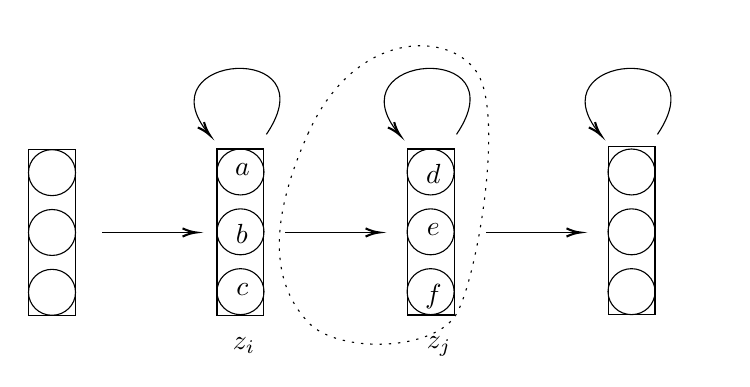
\begin{tikzpicture}[x=0.75pt,y=0.75pt,yscale=-0.6,xscale=0.6]
%uncomment if require: \path (0,265); %set diagram left start at 0, and has height of 265

%Shape: Ellipse [id:dp6772671720162915] 
\draw   (5.58,155.25) .. controls (5.58,145.06) and (14.04,136.8) .. (24.47,136.8) .. controls (34.9,136.8) and (43.35,145.06) .. (43.35,155.25) .. controls (43.35,165.44) and (34.9,173.7) .. (24.47,173.7) .. controls (14.04,173.7) and (5.58,165.44) .. (5.58,155.25) -- cycle ;
%Shape: Ellipse [id:dp7641461477821168] 
\draw   (5.58,107.21) .. controls (5.58,97.02) and (14.04,88.75) .. (24.47,88.75) .. controls (34.9,88.75) and (43.35,97.02) .. (43.35,107.21) .. controls (43.35,117.4) and (34.9,125.66) .. (24.47,125.66) .. controls (14.04,125.66) and (5.58,117.4) .. (5.58,107.21) -- cycle ;
%Shape: Ellipse [id:dp6352595087302537] 
\draw   (5.58,203.3) .. controls (5.58,193.11) and (14.04,184.85) .. (24.47,184.85) .. controls (34.9,184.85) and (43.35,193.11) .. (43.35,203.3) .. controls (43.35,213.49) and (34.9,221.75) .. (24.47,221.75) .. controls (14.04,221.75) and (5.58,213.49) .. (5.58,203.3) -- cycle ;
%Shape: Ellipse [id:dp08378668243039988] 
\draw   (156.93,154.72) .. controls (156.93,144.53) and (165.39,136.27) .. (175.82,136.27) .. controls (186.25,136.27) and (194.7,144.53) .. (194.7,154.72) .. controls (194.7,164.91) and (186.25,173.17) .. (175.82,173.17) .. controls (165.39,173.17) and (156.93,164.91) .. (156.93,154.72) -- cycle ;
%Shape: Ellipse [id:dp48928733013960746] 
\draw   (156.93,106.67) .. controls (156.93,96.48) and (165.39,88.22) .. (175.82,88.22) .. controls (186.25,88.22) and (194.7,96.48) .. (194.7,106.67) .. controls (194.7,116.86) and (186.25,125.12) .. (175.82,125.12) .. controls (165.39,125.12) and (156.93,116.86) .. (156.93,106.67) -- cycle ;
%Shape: Ellipse [id:dp42200756269881223] 
\draw   (156.93,202.76) .. controls (156.93,192.57) and (165.39,184.31) .. (175.82,184.31) .. controls (186.25,184.31) and (194.7,192.57) .. (194.7,202.76) .. controls (194.7,212.96) and (186.25,221.22) .. (175.82,221.22) .. controls (165.39,221.22) and (156.93,212.96) .. (156.93,202.76) -- cycle ;
%Straight Lines [id:da45440260704258306] 
\draw    (64.93,155.25) -- (138.24,155.25) ;
\draw [shift={(140.24,155.25)}, rotate = 180] [color={rgb, 255:red, 0; green, 0; blue, 0 }  ][line width=0.75]    (10.93,-3.29) .. controls (6.95,-1.4) and (3.31,-0.3) .. (0,0) .. controls (3.31,0.3) and (6.95,1.4) .. (10.93,3.29)   ;
%Curve Lines [id:da7444479405518811] 
\draw    (196.61,76.48) .. controls (248.16,0.58) and (96.42,11.3) .. (150.34,76.1) ;
\draw [shift={(151.16,77.08)}, rotate = 229.4] [color={rgb, 255:red, 0; green, 0; blue, 0 }  ][line width=0.75]    (10.93,-3.29) .. controls (6.95,-1.4) and (3.31,-0.3) .. (0,0) .. controls (3.31,0.3) and (6.95,1.4) .. (10.93,3.29)   ;
%Straight Lines [id:da24768191363471126] 
\draw    (211.91,155.25) -- (285.21,155.25) ;
\draw [shift={(287.21,155.25)}, rotate = 180] [color={rgb, 255:red, 0; green, 0; blue, 0 }  ][line width=0.75]    (10.93,-3.29) .. controls (6.95,-1.4) and (3.31,-0.3) .. (0,0) .. controls (3.31,0.3) and (6.95,1.4) .. (10.93,3.29)   ;
%Shape: Ellipse [id:dp19504276935561737] 
\draw   (309.6,154.72) .. controls (309.6,144.53) and (318.05,136.27) .. (328.48,136.27) .. controls (338.91,136.27) and (347.37,144.53) .. (347.37,154.72) .. controls (347.37,164.91) and (338.91,173.17) .. (328.48,173.17) .. controls (318.05,173.17) and (309.6,164.91) .. (309.6,154.72) -- cycle ;
%Shape: Ellipse [id:dp24864862911268681] 
\draw   (309.6,106.67) .. controls (309.6,96.48) and (318.05,88.22) .. (328.48,88.22) .. controls (338.91,88.22) and (347.37,96.48) .. (347.37,106.67) .. controls (347.37,116.86) and (338.91,125.12) .. (328.48,125.12) .. controls (318.05,125.12) and (309.6,116.86) .. (309.6,106.67) -- cycle ;
%Shape: Ellipse [id:dp602064917056562] 
\draw   (309.6,202.76) .. controls (309.6,192.57) and (318.05,184.31) .. (328.48,184.31) .. controls (338.91,184.31) and (347.37,192.57) .. (347.37,202.76) .. controls (347.37,212.96) and (338.91,221.22) .. (328.48,221.22) .. controls (318.05,221.22) and (309.6,212.96) .. (309.6,202.76) -- cycle ;
%Curve Lines [id:da1031770944487953] 
\draw    (349.28,76.48) .. controls (400.83,0.58) and (249.08,11.3) .. (303,76.1) ;
\draw [shift={(303.83,77.08)}, rotate = 229.4] [color={rgb, 255:red, 0; green, 0; blue, 0 }  ][line width=0.75]    (10.93,-3.29) .. controls (6.95,-1.4) and (3.31,-0.3) .. (0,0) .. controls (3.31,0.3) and (6.95,1.4) .. (10.93,3.29)   ;
%Straight Lines [id:da6790996887022185] 
\draw    (373.24,155.25) -- (446.55,155.25) ;
\draw [shift={(448.55,155.25)}, rotate = 180] [color={rgb, 255:red, 0; green, 0; blue, 0 }  ][line width=0.75]    (10.93,-3.29) .. controls (6.95,-1.4) and (3.31,-0.3) .. (0,0) .. controls (3.31,0.3) and (6.95,1.4) .. (10.93,3.29)   ;
%Shape: Ellipse [id:dp6867908324709058] 
\draw   (470.93,154.72) .. controls (470.93,144.53) and (479.39,136.27) .. (489.82,136.27) .. controls (500.25,136.27) and (508.7,144.53) .. (508.7,154.72) .. controls (508.7,164.91) and (500.25,173.17) .. (489.82,173.17) .. controls (479.39,173.17) and (470.93,164.91) .. (470.93,154.72) -- cycle ;
%Shape: Ellipse [id:dp11196197505608363] 
\draw   (470.93,106.67) .. controls (470.93,96.48) and (479.39,88.22) .. (489.82,88.22) .. controls (500.25,88.22) and (508.7,96.48) .. (508.7,106.67) .. controls (508.7,116.86) and (500.25,125.12) .. (489.82,125.12) .. controls (479.39,125.12) and (470.93,116.86) .. (470.93,106.67) -- cycle ;
%Shape: Ellipse [id:dp0016693710735093958] 
\draw   (470.93,202.76) .. controls (470.93,192.57) and (479.39,184.31) .. (489.82,184.31) .. controls (500.25,184.31) and (508.7,192.57) .. (508.7,202.76) .. controls (508.7,212.96) and (500.25,221.22) .. (489.82,221.22) .. controls (479.39,221.22) and (470.93,212.96) .. (470.93,202.76) -- cycle ;
%Curve Lines [id:da2339937869181159] 
\draw    (510.61,76.48) .. controls (562.16,0.58) and (410.42,11.3) .. (464.34,76.1) ;
\draw [shift={(465.16,77.08)}, rotate = 229.4] [color={rgb, 255:red, 0; green, 0; blue, 0 }  ][line width=0.75]    (10.93,-3.29) .. controls (6.95,-1.4) and (3.31,-0.3) .. (0,0) .. controls (3.31,0.3) and (6.95,1.4) .. (10.93,3.29)   ;
%Shape: Polygon Curved [id:ds1112844353439364] 
\draw  [dash pattern={on 0.84pt off 2.51pt}] (230.03,75.9) .. controls (268.03,-8.76) and (344.7,-6.76) .. (366.03,27.24) .. controls (387.37,61.24) and (366.7,187.24) .. (350.03,219.24) .. controls (333.37,251.24) and (254.03,252.57) .. (230.7,227.9) .. controls (207.37,203.24) and (192.03,160.57) .. (230.03,75.9) -- cycle ;
%Shape: Rectangle [id:dp8143917355569943] 
\draw   (43.35,88.53) -- (5.37,88.53) -- (5.37,221.75) -- (43.35,221.75) -- cycle ;
%Shape: Rectangle [id:dp4298068501555119] 
\draw   (194.47,88.22) -- (156.93,88.22) -- (156.93,221.86) -- (194.47,221.86) -- cycle ;
%Shape: Rectangle [id:dp3487560630191522] 
\draw   (347.85,88.22) -- (309.6,88.22) -- (309.6,221.53) -- (347.85,221.53) -- cycle ;
%Shape: Rectangle [id:dp5041089294978152] 
\draw   (508.7,86.05) -- (471.17,86.05) -- (471.17,221.22) -- (508.7,221.22) -- cycle ;

% Text Node
\draw (169.33,98.07) node [anchor=north west][inner sep=0.75pt]    {$a$};
% Text Node
\draw (170,146.73) node [anchor=north west][inner sep=0.75pt]    {$b$};
% Text Node
\draw (170.33,194.4) node [anchor=north west][inner sep=0.75pt]    {$c$};
% Text Node
\draw (322.67,98.07) node [anchor=north west][inner sep=0.75pt]    {$d$};
% Text Node
\draw (323.33,146.07) node [anchor=north west][inner sep=0.75pt]    {$e$};
% Text Node
\draw (322,195.07) node [anchor=north west][inner sep=0.75pt]    {$f$};
% Text Node
\draw (167.64,237.44) node [anchor=north west][inner sep=0.75pt]    {$z_{i}$};
% Text Node
\draw (323.3,236.78) node [anchor=north west][inner sep=0.75pt]    {$z_{j}$};


\end{tikzpicture}

	
	\end{figure}
	\[
	W = \kbordermatrix{
    & a & b & c & d & e & f \\
    d & W_{da} & W_{db} & W_{dc} & 0 & W_{de} & W_{df} \\
    e & W_{ea} & W_{eb} & W_{ec} & W_{ed} & 0 & W_{ef} \\
    f & W_{fa} & W_{fb} & W_{fc} & W_{fd} & W_{fe} & 0}
	\]
	

\end{frame}

\begin{frame}{Questions}
	\begin{itemize}[label=--]
	\item Input: now converting signal to Bernoulli spikes, and then feeding them to layer 0.
	\end{itemize}
\end{frame}

%\begin{frame}{Outer loop (Level 0)}
%	
%\begin{algorithmic}
%\State $W \gets W_0$
%\State $D_T, D_V \gets \text{load\_data}$
%\For{$e$ in $[0, E]$}
%
%	\State $B_T \gets \text{make\_batch}(D_T)$
%	\State $(E_T, \Delta W) \gets \text{train\_on\_batch}(B_T)$
%	\State $W \gets \text{update\_weight}(\Delta W)$
%	\State $B_V \gets \text{make\_batch}(D_V)$
%	\State $E_V \gets \text{train\_on\_batch}(B_T)$
%	\If{$E_V < E_{V_\text{opt}}$}
%	\State $W_\text{opt} \gets W$
%	\State $E_{V_\text{opt}} \gets E_V$
%	\EndIf
%	
%\EndFor
%\end{algorithmic}
%\end{frame}
%
%\begin{frame}{Batch loop (Level 1)}
%	
%\begin{algorithmic}
%\State $E \gets 0$
%\State $\Delta W \gets {(\Delta W)}_0$
%\For{$(X, Y)$ in $B$}
%
%	\State $X, Y \gets \text{repeat}((X, Y))$
%	\State $M \gets \text{eprop}(X, W)$
%	\State $E \gets E + \text{get\_error}(M, Y)$	
%\EndFor
%
%\State $\Delta W \gets \text{update\_gradients}(E, M, \Delta W)$
%\State $L \gets $
%\end{algorithmic}
%\end{frame}


\end{document}
